\section{Efficiently updatable neural networks}

NNUE (\reflectbox{NNUE} Efficiently updatable neural network) is a neural network architecture that allows for very fast subsequent evaluations when changes in the input are minimal. It was invented for Shogi by Yu Nasu in 2018 \cite{nnue:2018}, later adapted to Chess for use in Stockfish in 2019. Most of the information described in this chapter can be found in the excellent Stockfish NNUE documentation \cite{nnue-pytorch}. \\

NNUE operates on the following principles:

\begin{itemize}
    \item \textbf{Input sparsity}: The network should have a relatively low amount of non-zero inputs, determined by the chosen feature set. The presented feature sets have between 0.1\% and 2\% of non-zero inputs for a typical position. Having a low amount of non-zero inputs places a low upper bound on the time required to evaluate the network in its entirety, which can happen using some feature sets like \featureset{King-All} that triggers a complete refresh when the king is moved.
    \item \textbf{Efficient updates}: From one evaluation to the next, the number of inputs changes should be as low as possible. This allows for the most expensive part of the network to be efficiently updated, instead of recomputed from scratch.
    \item \textbf{Simple architecture}: The network should be composed of a few and simple operators, that can be efficiently implemented with low-precision arithmetic in integer domain using CPU hardware (quantization).

\end{itemize}

There is a tradeoff between inference time and quality of the predictions, which affect the amount of nodes evaluated. If the inference is faster, more nodes can be evaluated thus reaching deeper in the search tree. Having higher quality predictions, which usually comes with a more complex model and/or feature set, can make stronger moves with shallower searches, and may improve prunning.

Models must be so much better to compensate the slowdown in inference when using bigger models or more complex feature sets. This is a tradeoff that will appear further in the experiments.

\subsection{Layers}

For this thesis, I have chosen to use a very simple NNUE architecture, which consist of two linear (fully connected) layers and clipped ReLU activations. In the literature, there are other architectures that make use of polling layers, sigmoid activations and others. Since this work is about experimenting with feature sets, I have chosen to stick with something simple that has been proven to achieve good results.

\paragraph[short]{Linear layer} A linear layer is a matrix multiplication followed by a bias addition. It takes \textbf{in\_features} input values and produces \textbf{out\_features} output values. The operation is $\bm{y} = \bm{W} \bm{x} + \bm{b}$, where:

\begin{enumerate}
\item $\bm{x}$ the input column vector of shape \textbf{in\_features}.
\item $\bm{W}$ the weight matrix of shape (\textbf{out\_features}, \textbf{in\_features}).
\item $\bm{b}$ the bias column vector of shape \textbf{out\_features}.
\item $\bm{y}$ the output column vector of shape \textbf{out\_features}.
\end{enumerate}

If we call $\bm{A_i}$ the $i$-th column of the weight matrix $\bm{W}$, the operation $\bm{W} \bm{x}$ can be simplified to \enquote{if $\bm{x_i}$ is not zero, take the column $\bm{A_i}$, multiply it by $\bm{x_i}$ and add it to the result}. This means that we can skip the processing of columns that have a zero input, as depicted in figure \ref{fig:linear_comparison}.

\begin{figure}[H]
\centering
\subfloat[\centering Linear layer]{{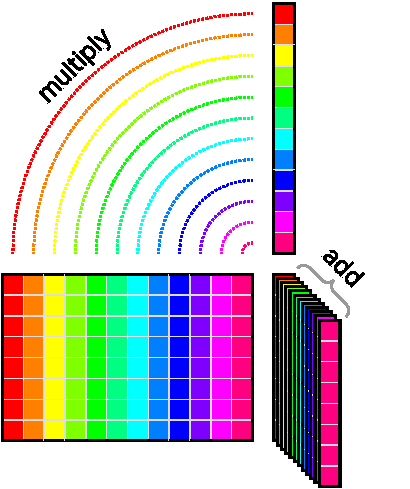
\includegraphics[width=5cm]{../assets/nnue/mv.pdf} }}%
\qquad
\subfloat[\centering Linear layer with sparse inputs]{{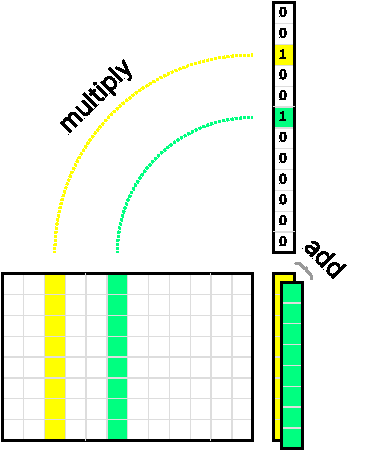
\includegraphics[width=5cm]{../assets/nnue/mvs.pdf} }}%
\caption{Linear layer operation comparison. Figures from \cite{nnue-pytorch}.}
\label{fig:linear_comparison}
\end{figure}

In the case of the first layer, the input is a very sparse one-hot encoded vector. This means that very few columns will have to be processed and the multiplication can be skipped altogether, due all inputs being either 0 or 1. Skipping the multiplication reduces the operations to only additions and subtractions.

\paragraph[short]{Clipped ReLU} This is a simple activation that clips the output in the range $[0, 1]$. The operation is $\bm{y=\min(\max(x,0),1)}$.
The output of this activation function is the input for the next layer, and because of the aggresive \textit{quantization} that will be described later, it is necessary to restrain the values so it does not overflow. \\

\subsection{Efficient updates}

When running a depth-first search algorithm, the state of the position is updated every time the algorithm \textit{makes} and \textit{unmakes} moves, usually before and after the recursion.
NNUEs are designed to work with this kind of search, since every time the algorithm \textit{makes} (or \textit{unmakes}) a move, the changes in the position are minimal (at most two pieces are affected in \featureset{All}), meaning that the amount of features becoming active or inactive is minimal as well. This is depicted in figure \ref{fig:updates_tree}.

\begin{figure}[H]
\centering
\storechessboardstyle{3x3}{tinyboard,maxfield=c3,margin=false,showmover=false,hlabel=true,vlabel=true,pgfstyle=color,color=blue}
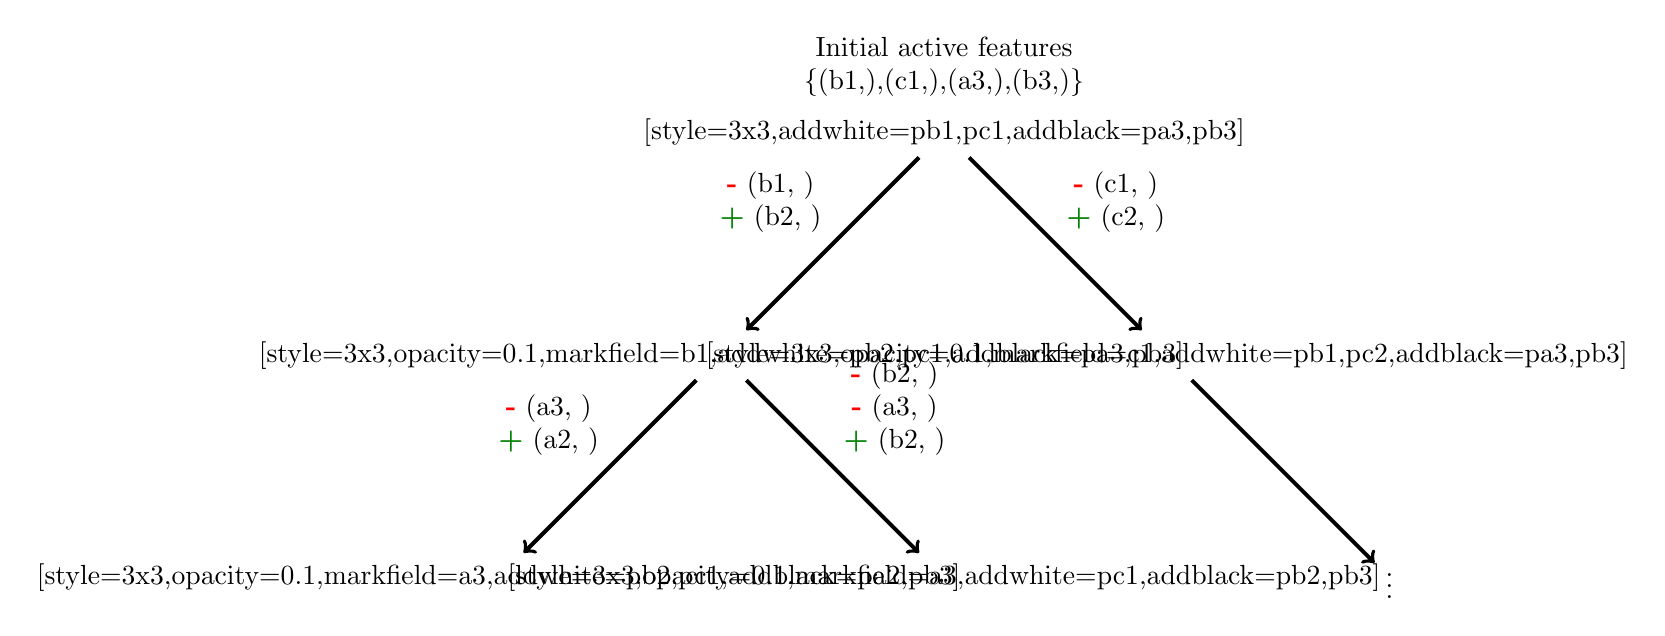
\begin{tikzpicture}[
    node distance=4cm,
    line width=0.5mm,
    auto
]

    \node[label={[align=center]Initial active features \\ \{(b1,\white),(c1,\white),(a3,\black),(b3,\black)\}}] (A) {\chessboard[style=3x3,addwhite={pb1,pc1},addblack={pa3,pb3}]};

    % childs of A
    \node (B) [below left of=A] {\chessboard[style=3x3,opacity=0.1,markfield={b1},addwhite={pb2,pc1},addblack={pa3,pb3}]};
    \node (C) [below right of=A] {\chessboard[style=3x3,opacity=0.1,markfield={c1},addwhite={pb1,pc2},addblack={pa3,pb3}]};

    % childs of B
    \node (D) [below left of=B] {\chessboard[style=3x3,opacity=0.1,markfield={a3},addwhite={pb2,pc1},addblack={pa2,pb3}]};
    \node (E) [below right of=B] {\chessboard[style=3x3,opacity=0.1,markfield={a3},addwhite={pc1},addblack={pb2,pb3}]};

    % childs of C
    \node (F) [below right of=C] {\vdots};

    % arrows of A
    \path[<-] (B) edge node[align=center] {\textbf{{\color{Red}-}} (b1, \white) \\ \textbf{{\color{Green}+}} (b2, \white)} (A);
    \path[->] (A) edge node[align=center] {\textbf{{\color{Red}-}} (c1, \white) \\ \textbf{{\color{Green}+}} (c2, \white)} (C);
    
    % arrows of B
    \path[<-] (D) edge node[align=center] {\textbf{{\color{Red}-}} (a3, \black) \\ \textbf{{\color{Green}+}} (a2, \black)} (B);
    \path[->] (B) edge node[align=center] {\textbf{{\color{Red}-}} (b2, \white) \\ \textbf{{\color{Red}-}} (a3, \black) \\ \textbf{{\color{Green}+}} (b2, \black)} (E);

    % arrows of C
    \path[<-] (F) edge node[align=center] {} (C);

\end{tikzpicture}
\caption{Partial tree of feature updates (\textcolor{Red}{removals} and \textcolor{Green}{additions}) for $(\featureset{Squares} \times \featureset{Colors})$ (white's point of view) in a simplified 3x3 pawn-only board.}
\label{fig:updates_tree}
\end{figure}

To take advantage of this during search, instead of computing all the features active in a position and then evaluate the network in its entirety, we can \textbf{accumulate} the output of the first linear layer and update it with when the position changes. Linear layers can be computed adding the corresponding columns of the weight matrix into the output, so when a feature becomes active or inactive, we can add or subtract the corresponding column to the output. When the evaluation is needed, only the next layers (usually small) have to be computed. \\

Recall that the way I defined feature sets, they always encode the position from one white's point of view. This means that its not possible to use the same \textbf{accumulator} for both players. So when running the search, we have to keep two accumulators, one for white and one for black, where the black board is flipped and has the colors swapped to match the point of view.

% [agregar grafico de black → white board → encode, para mostrar como se flipea / swapea. arriba el white → encode; poner los features activos quizas?]

%\begin{figure}[h]
%\centering
%
%\begin{tabular}{ccccc}
%
%\raisebox{-7ex}{\chessboard[
%    setfen=2Qb4/5pk1/p5p1/1pp3Pp/3qPp1P/P7/1PP1B3/1K6 w - - 1 29,
%    tinyboard,
%]}
%
%&
%
%&
%
%
%&
%
%$\xrightarrow{\text{encode}}$
%
%&
%
%Features
%
%\\
%
%\raisebox{-7ex}{\chessboard[
%    setfen=2Qb4/5pk1/p5p1/1pp3Pp/3qPp1P/P7/1PP1B3/1K6 b - - 1 29,
%    tinyboard,
%]}
%
%&
%
%$\xrightarrow{\text{flip vertically}}$
%
%&
%
%\raisebox{-7ex}{\chessboard[
%    setfen=2Qb4/5pk1/p5p1/1pp3Pp/3qPp1P/P7/1PP1B3/1K6 b - - 1 29,
%    tinyboard,
%]}
%
%&
%
%$\xrightarrow{\text{swap colors}}$
%
%&
%
%\raisebox{-7ex}{\chessboard[
%    setfen=2qB4/5PK1/P5P1/1PP3pP/3QpP1p/p7/1pp1b3/1k6 w - - 1 29,
%    tinyboard,
%]}
%
%
%\end{tabular}
%\end{figure}


During search, the first layer is replaced by two accumualtors to take advantage of this. Figure \ref{fig:incr_update} depicts how the output of both accumulators is concatenated depending on which player is moving, to later be passed through the rest of the network which is computed as usual. 

\begin{figure}[H]
\centering
\makebox[\textwidth]{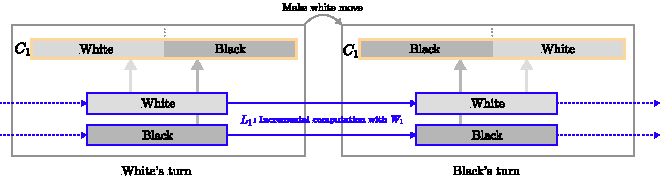
\includegraphics[width=\textwidth]{../assets/nnue/incremental_update.pdf}}
\caption{Concatenation of the first layer's output after a move is made. Inspired in a CPW figure.}
\label{fig:incr_update}
\end{figure}

\subsection{Network}

The network will be composed of three linear layers $L_1$ through $L_3$, each but the last one followed by a clipped ReLU activation $C_1$ and $C_2$. The network has two inputs: it takes the encoding (feature set) of a position from each player's point of view. Each encoding is passed through the same $L_1$ layer (same weights) and then the output is concatenated before passing it through the rest of the network. The first layer can be seen as a feature transformer, and it must share weights to allow for efficient updates. The network can be described as follows: \\

$\bm{N}$: number of features in the feature set

\begin{enumerate}
\itemsep-0.2em
\item $L_1 \times 2$: Linear from $\bm{N}$ to $\bm{M}$ ($\bm{W_1}$ weight, $\bm{b_1}$ bias)
\item $C_1$: Clipped ReLU of $\bm{2 * M}$
\itemsep0.2em
\item $L_2$: Linear from $\bm{2 * M}$ to $\bm{O}$ ($\bm{W_2}$ weight, $\bm{b_2}$ bias)
\itemsep-0.2em
\item $C_2$: Clipped ReLU of $\bm{O}$
\itemsep0.2em
\item $L_3$: Linear from $\bm{O}$ to $\bm{1}$ ($\bm{W_3}$ weight, $\bm{b_3}$ bias)
\end{enumerate}


The size of each layer is not fixed since it is a hyperparameter I will experiment with. The network architecture is depicted in figure \ref{fig:network}, with example parameters.

\begin{figure}[H]
\centering
\makebox[\textwidth]{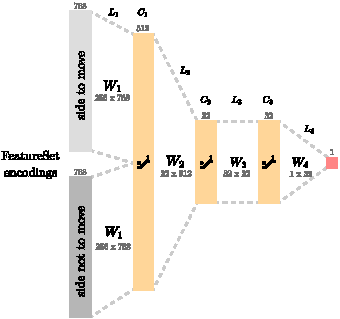
\includegraphics[width=10cm]{../assets/nnue/network.pdf}}
\caption{Neural network architecture with $\bm{N}=768$, $\bm{M}=256$, $\bm{O}=32$. Not to scale.}
\label{fig:network}
\end{figure}

\subsection{Quantization}

% https://github.com/official-stockfish/nnue-pytorch/blob/master/docs/nnue.md#quantization

Quantization is the process of converting the operations and parameters of a network to a lower precision. It is a step performed after all training has been done, which do happen in float domain. Floating point operations are too slow to achieve acceptable performance, as it sacrifices too much speed. This was necessary to implement to have a working engine.

Quantizing the network to integer domain will inevitable introduce some error, but it far outweights the performance gain. In general, the deeper the network, the more error is accumulated, but since NNUEs are very shallow by design, the error is negligible. At the end of the chapter I do an analysis of the error introduced by quantization.

Since the objective is to take advantage of modern CPUs that allow doing low-precision integer arithmetic in parallel with 8, 16, 32 or even 64 8-bit integer values at a time, we want to use the smallest integer type possible everywhere, to process more values at once.

\newpage
\subsubsection{Stockfish quantization scheme}

\def\int#1{\texttt{int#1}}

In this thesis, I will use the same quantization scheme used in the engine Stockfish \cite{nnue-pytorch}, due its simplicity and it has been battle tested. It uses \int{8} $[-128, 127]$ for inputs and weights, and \int{16} $[-32768, 32767]$ where \int{8} does not fit the range of values we need.
To convert the float values to integer, we need to multiply the weights and biases by some constant to translate them to a different range of values. Each layer is different, so I'll go through each one.

%\begin{figure}[H]
%\centering
%\makebox[\textwidth]{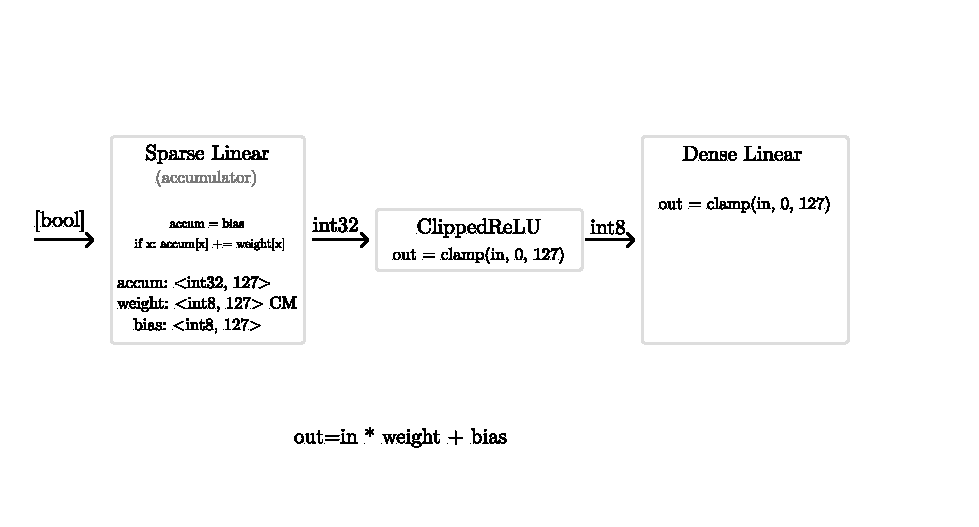
\includegraphics[width=\textwidth]{../%assets/nnue/quantization.pdf}}
%\caption{Simplified network showcasing all layers with %quantization values}
%\label{fig:quantization}
%\end{figure}

\paragraph[short]{Input} In float domain inputs are either $0.0$ or $1.0$, and since they are quantized to \int{8} we must scale them by $s_a=127$ (activation scale), so inputs are either $0$ or $127$. During inference, the input values are not computed since the first layer is an accumulator. However it is important to note that the rows being accumulated are scaled by $s_a=127$.

\paragraph[short]{ClippedReLU} The output of the activation in float domain is in the range $[0, 1]$ and we want to use \int{8} in the quantized version, so we can multiply by $s_a=127$ and clamp in the range [0, 127]. The input data type may change depending on the previous layer: if it comes from the accumulator, it will be \int{32}, and if it comes from a linear layer, it will be \int{16}.

% \paragraph[short]{Input} Since we are using accumualtors, there is not a real input to the model.
% Inputs are quantized to 8 bits, so the range of values is $-128..127$. Since the inputs are hot encoded, the float values are 0.0 or 1.0, so the quantized values are either 0 or 127.

\paragraph[short]{Accumulator (L1)}



The purpose of this layer is to accumulate rows of the first layer's weight matrix, which is stored in \int{16}. The values are stored in column-major order so a single row is contiguous in memory. Since we are accumulating potentially hundreds of values which are stored in \int{16} and scaled by $s_a=127$, we must accumulate in \int{32} to avoid overflows. The output of this layer will be the input for the ClippedReLU activation.

\paragraph[short]{Linear layer (L2 and L3)} The input to this layer will be scaled to the activation range because it takes the output of the previous ClippedReLU activation: $s_a \bm{x}$. We want the output to also be scaled to the activation range so it can be passed to the next: $s_a \bm{y}$.

To convert the weights to \int{8}, we must scale them by some factor $s_W=64$ (value used in Stockfish, efficient in SIMD because is just a shift): $s_W \bm{W}$. The value $s_W$ depends on how much precision we want to keep, but if it is too large the weights will be limited in magnitude. The range of the weights in floating point is then determined by \mbox{$\pm \frac{s_a}{s_W}=\frac{127}{64}=1.984375$}, and to make sure weights don't overflow, it is necessary to clip them to this range during training. The value $s_W$ also determinates the minimum representable weight step, which is $\frac{1}{s_W}=\frac{1}{64}=0.015625$.

The linear layer operation with the scaling factors applied looks like:

\begin{equation}
\begin{aligned}
s_a s_W \bm{y} &= (s_W \bm{W}) (s_a \bm{x}) + s_a s_W \bm{b} \\
\end{aligned}
\end{equation}
\begin{equation}
\begin{aligned}
s_a \bm{y} &= \frac{(s_W \bm{W}) (s_a \bm{x}) + s_a s_W \bm{b}}{s_W} \\
\end{aligned}
\end{equation}

From that equation we can extract that, to obtain the result we want, which is the output of the layer scaled to the activation range ($s_a \bm{y}$), we must divide the result of the operation by $s_W$ (2). Also that the bias must be scaled by $(s_a s_W)$. \\

The last linear layer (L3) is a bit different since there is no activation afterwards, so we don't want any scalings at all:

\begin{equation}
\begin{aligned}
\bm{y} = \frac{(s_W \bm{W}) (s_a \bm{x}) + s_a s_W \bm{b}}{s_a s_W}
\end{aligned}
\end{equation}

% no se tiene el mismo problema que en el accumulator layer porque la multiplicacion en SIMD se hace en 32 bits (osea sin hacer overflow), para despues aplicar clippedrelu a eso.

\subsection{Implementation}

The Stockfish repository provides an AVX2 implementation of the mathematical operations in C++. They have been carefully ported to Rust for this thesis. The implementation was thoroughly tested using the Pytorch model as reference (output match).

\subsubsection{Quantization error}

To make sure the quantization is working as expected, I compared the actual output of the quantized model (in Rust) with the float model (in Python) by running them in thousands of positions.

% https://discord.com/channels/435943710472011776/718853716266188890/802646172388294706

\begin{figure}[H]
\centering
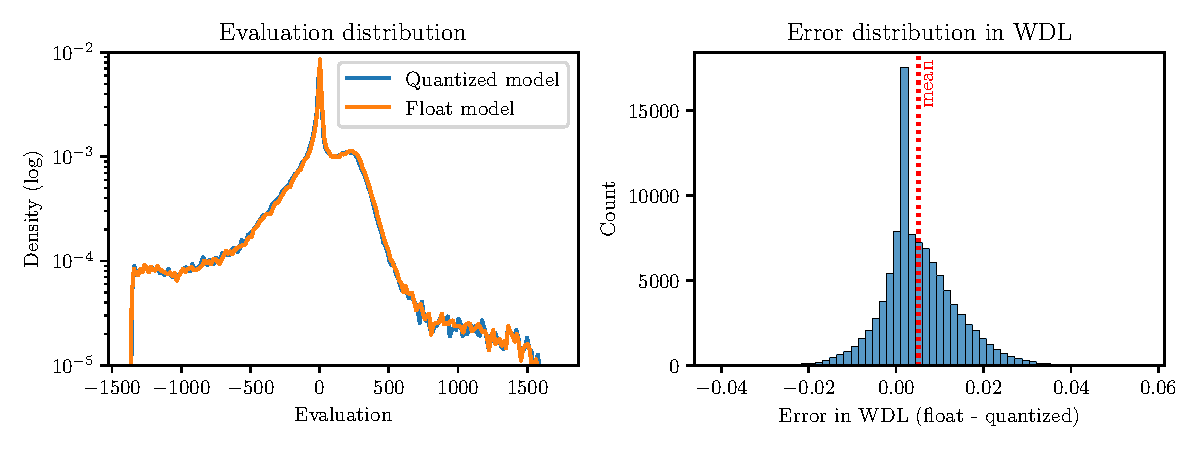
\includegraphics[width=\textwidth]{./dynamic/output/quant_errors.pdf}
\caption{Comparison between the float model and the quantized model. $N=100000$}
\label{fig:quant_errors}
\end{figure}

In figure \ref{fig:quant_errors} we can see that the distribution of the evaluation of both models is almost identical, indicating that the implementation is correct.

To measure the error introduced it is better to do it in WDL-space, since we can make sense of values in that space. The errors are near zero, and almost all errors are within 0.03 units, which is a 3\% difference in winrate. The Stockfish team has reported that errors in quantization up to 5\% do not affect the engine's strength \footnote{\href{https://discord.com/channels/435943710472011776/718853716266188890/814260897040039977}{Sopel's message on Discord about this} (official Stockfish server).}.
